\chapter{Pruebas y Resultados}
\label{cap:7}

En el presente capítulo se describen las pruebas de campo realizadas y los resultados obtenidos. Un primer grupo de pruebas tuvo por objetivo determinar los valores más adecuados para los parámetros utilizados en la recolección de FCD, tanto en el reconocimiento de actividad como en la toma de localizaciones. Otro grupo de pruebas se realizó con el objetivo determinar la efectividad del sistema implementado, para ello se verificó la tasa de acierto del algoritmo de MM y se analizaron los datos obtenidos para determinar las horas pico y los días con mayor flujo de tráfico.

Debido a la complejidad y a la gran cantidad de variables intervinientes en el funcionamiento del sistema se optó por realizar pruebas de campo en lugar de utilizar simulaciones. Para las pruebas se utilizaron dispositivos móviles de diversa gama y se realizaron tanto en vehículos de transporte público, como en vehículos privados, también se analizaron los datos generados por usuarios reales del sistema. 

\section{Deducción de parámetros para FCD}

En la recolección de FCD se utiliza un esquema de detección de actividad que permite a la aplicación registrar las localizaciones del usuario únicamente cuando se encuentra en un vehículo en movimiento. Para ello, la aplicación móvil verifica periódicamente cuál es la actividad que está realizando el usuario en base a las lecturas de los sensores del dispositivo. 

El intervalo de tiempo en el que se realiza la verificación de actividad se denomina \emph{intervalo de reconocimiento} y determina qué tan rápido se detecta el movimiento para iniciar o finalizar el rastreo. Es importante tener en cuenta que mientras más corto es el intervalo, mayor es el consumo de batería debido a que el dispositivo móvil debe procesar más frecuentemente las muestras de los sensores. Para determinar el valor apropiado para el intervalo de reconocimiento se realizaron pruebas empíricas con diferentes valores obteniéndose para cada uno de ellos el tiempo promedio que tarda en detectarse el movimiento. 

La \Cref{tab:prom_intervalo_reconocimiento} muestra el tiempo promedio que la aplicación tarda en detectar el movimiento e iniciar la toma de localizaciones para varios valores del intervalo de reconocimiento. Como se puede apreciar, un intervalo de reconocimiento corto ayuda a iniciar más rápidamente la toma de localizaciones. En base a las pruebas realizadas el intervalo de reconocimiento seleccionado es de 30 segundos, por ser el intervalo más largo que presenta un tiempo de respuesta que no causa pérdidas significativas en el trayecto rastreado.


\begin{table}[h]
  \centering
	\begin{tabular}{ccccc}
	\toprule
	Intervalo (s) & Nº de recorridos & En bus (min.) & En auto (min.) & Ambos (min.) \\
	\midrule
	15            & 30       & 1.55         & 1.25            & 1.40         \\
	30            & 30       & 1.64         & 1.75            & 1.71         \\
	45            & 30       & 2.59         & 2.05            & 2.32         \\
	60            & 30       & 4.37         & 2.75            & 3.66         \\
	\bottomrule
	\end{tabular}
  \caption{Tiempos promedio para inicio de rastreo}
  \label{tab:prom_intervalo_reconocimiento}
\end{table}


El reconocimiento de actividad también es utilizado para detener la toma de localizaciones cuando el usuario ya no se encuentra en un vehículo en movimiento. Se debe tener en cuenta que durante una trayectoria el vehículo puede detenerse momentáneamente debido a diversas causas, como ser un semáforo en rojo o una parada de bus. En estos casos la toma de localizaciones no debe ser erróneamente detenida porque se producirían cortes en la captura del trayecto. 

Para evitar cortes en el rastreo se introduce un \emph{tiempo de tolerancia} en el reconocimiento de actividad para detener el rastreo. Cada vez que se detecta el movimiento, se almacena el tiempo de detección y el rastreo no es detenido hasta que haya transcurrido el tiempo de tolerancia a partir de la última vez que se detectó movimiento. Se debe tener en cuenta también que un tiempo de tolerancia alto implica que se tardará más en detener el servicio de localización, lo que puede producir un impacto negativo en el consumo de batería.

El tiempo que el dispositivo estuvo rastreando al usuario puede ser menor al tiempo total que duró realmente el viaje. El porcentaje de tiempo que el dispositivo estuvo rastreando al usuario con respecto al tiempo total que duró el viaje se denomina \emph{tiempo efectivo de rastreo}. Los valores de tiempo de tolerancia e intervalo de reconocimiento en conjunto influyen en el tiempo efectivo de rastreo por lo que deben ser escogidos apropiadamente.

En la \Cref{tab:prom_tiempo_efectivo_rastreo} se muestran los resultados acerca del tiempo efectivo de rastreo observado para diferentes combinaciones de valores de intervalo de reconocimiento y de tiempo de tolerancia considerados. 

\begin{table}[h]
    \centering
	\begin{tabular}{ccccc}
    	\toprule
    	Intervalo (s) & Tolerancia (min.) & En bus (\%) & En auto (\%) & Ambos (\%) \\
    	\midrule
    	15            & 5                 & 89.31         & 93.67          & 91.49        \\
    	30            & 5                 & 85.86         & 91.56          & 88.71        \\
    	45            & 5                 & 83.34         & 89.32          & 86.33        \\
    	60            & 5                 & 80.83         & 87.73          & 84.24        \\
    	15            & 10                & 95.83         & 97.22          & 96.53        \\
    	30            & 10                & 94.44         & 96.11          & 95.28        \\
    	45            & 10                & 89.55         & 95.44          & 92.49        \\
    	60            & 10                & 83.33         & 93.89          & 88.61        \\
    	\bottomrule
	\end{tabular}
    \caption{Tiempos efectivos de rastreo}
    \label{tab:prom_tiempo_efectivo_rastreo}
\end{table}

De las pruebas realizadas puede notarse que con una tolerancia de 10 minutos combinada con un intervalo de reconocimiento de 30 segundos se obtienen coberturas del 95\%, seleccionándose dichos valores como apropiados para este trabajo.

\section{Verificación de efectividad de MM}

Para el MM se utiliza el algoritmo ST-Matching como se describe en \cref{implementacion_mm}. Este algoritmo recibe como entrada un conjunto de localizaciones correspondientes a una trayectoria seguida por un usuario, el intervalo de tiempo con el que se obtienen estos puntos se denomina \emph{intervalo de muestreo}. Si el intervalo es grande, se tiene un menor número de muestras para un periodo de tiempo dado y por ende un menor consumo de batería del dispositivo móvil. En cambio, para intervalos pequeños, se tiene un mayor número de muestras y un elevado consumo de batería. Para medir la efectividad del MM, se observa la cantidad de puntos que son correctamente asignados a las calles al estimar el camino real recorrido.

Las pruebas de MM consistieron en la observación de su efectividad con diferentes intervalos de muestreo. Los intervalos observados fueron de 30, 60 y 120 segundos, para cada intervalo se realizaron varios recorridos, se sumó la cantidad total de puntos recolectados y se comparó con la cantidad de puntos correctamente asignados. Los resultados obtenidos pueden ser apreciados en la \Cref{table:map_matching}. Para intervalos pequeños de toma localizaciones se tienen mejores resultados, con una leve diferencia a favor del intervalo de 30 segundos en comparación al intervalo de 60 segundos y con una diferencia un poco mayor en comparación al de 120 segundos. En base a estos resultados se decidió utilizar el intervalo de 60 segundos debido a que consume menos batería y produce resultados similares al intervalo de 30 segundos.

\begin{table}[h]
	\centering
	\begin{tabular}{cccc}
        \toprule
    	Intervalo (s) & Total de Puntos & Puntos Correctos & Tasa de Acierto (\%)\\
    	\midrule
    	30 & 120  & 111 & 93 \\
    	60 & 120 & 109 & 91 \\
    	120 & 120 & 106 & 88 \\ 
    	\bottomrule
	\end{tabular}
	\caption{Efectividad del MM} 
	\label{table:map_matching}
\end{table}

A continuación se presenta el desempeño del MM para un mismo recorrido utilizando los tres intervalos analizados. Se muestra con una línea roja el recorrido observado por el vehículo, y con una línea verde el recorrido aproximado después de realizar el MM. La \Cref{fig:mm_30s} corresponde a las muestras obtenidas utilizando un intervalo de muestreo de 30 segundos, las \Cref{fig:mm_1m,fig:mm_2m} corresponden a intervalos de 1 y 2 minutos respectivamente. Se puede observar que con intervalos más amplios, las localizaciones tomadas están más distanciadas entre si. Gracias al algoritmo de MM utilizado, el camino generado es prácticamente el mismo para todo los intervalos observados observadas.

\begin{figure}[!htb]
	\centering
	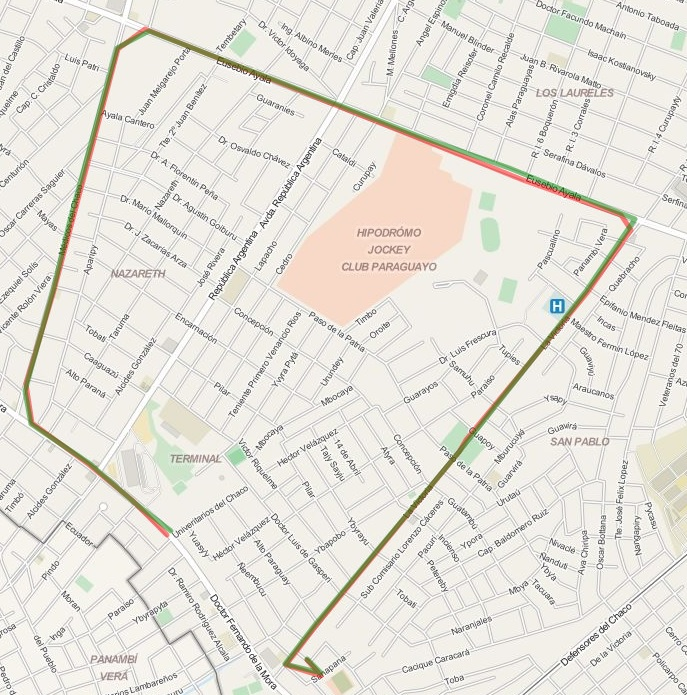
\includegraphics[width=0.7\textwidth]{capitulos/7/figuras/figura1.jpg}
	\caption{\label{fig:mm_30s} MM con intervalo de 30 segundos}	
\end{figure}

\begin{figure}[!htb]
	\centering
	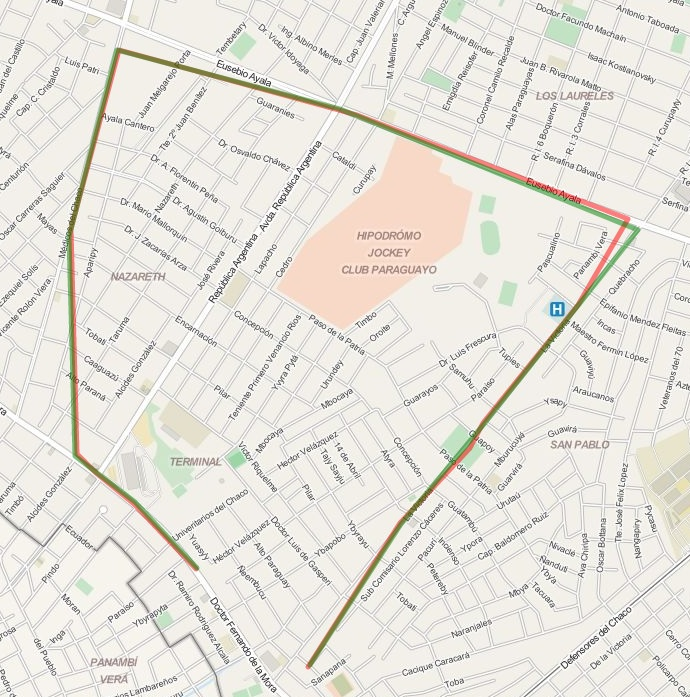
\includegraphics[width=0.7\textwidth]{capitulos/7/figuras/figura2.jpg}
	\caption{\label{fig:mm_1m} MM con intervalo de 1 minuto}	
\end{figure}

\begin{figure}[!htb]
	\centering
	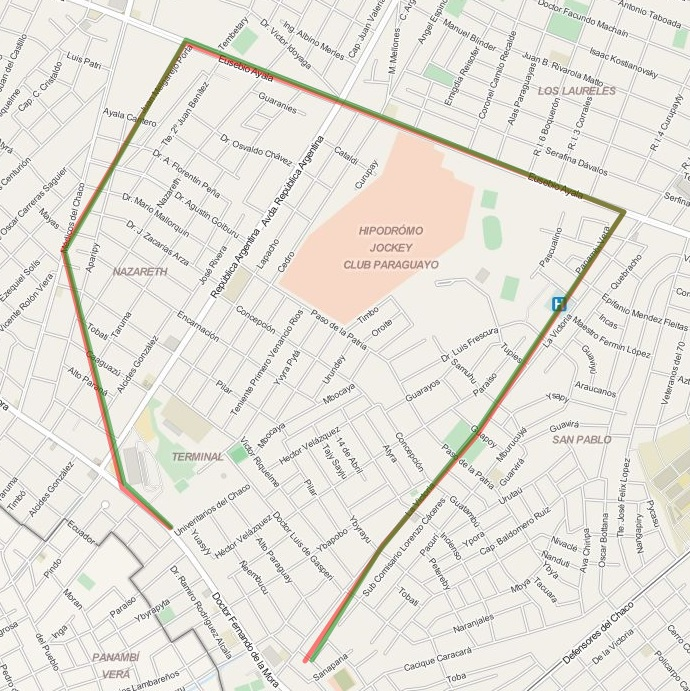
\includegraphics[width=0.7\textwidth]{capitulos/7/figuras/figura3.jpg}
	\caption{\label{fig:mm_2m} MM con intervalo de 2 minutos}	
\end{figure}

\section{Análisis de Tráfico}

Para realizar las pruebas de análisis de tráfico se distribuyó la aplicación Autotracks a través de Google Play\footnote{https://play.google.com/store} y se observaron los resultados obtenidos a durante un periodo de 5 semanas de uso de la aplicación. Durante ese periodo de tiempo un promedio de 212 usuarios utilizaron la aplicación diariamente, generando un total de 123419 puntos observados desde sus dispositivos móviles. Debido a que los usuarios pueden activar o desactivar los sensores de sus teléfonos, no se hace distinción entre los puntos obtenidos a través de GPS, Wifi o triangulación de antenas. En la \Cref{fig:cantidad_usuarios} se observa la cantidad de usuarios activos por día durante el periodo de prueba.

\begin{figure}[h]
	\centering
	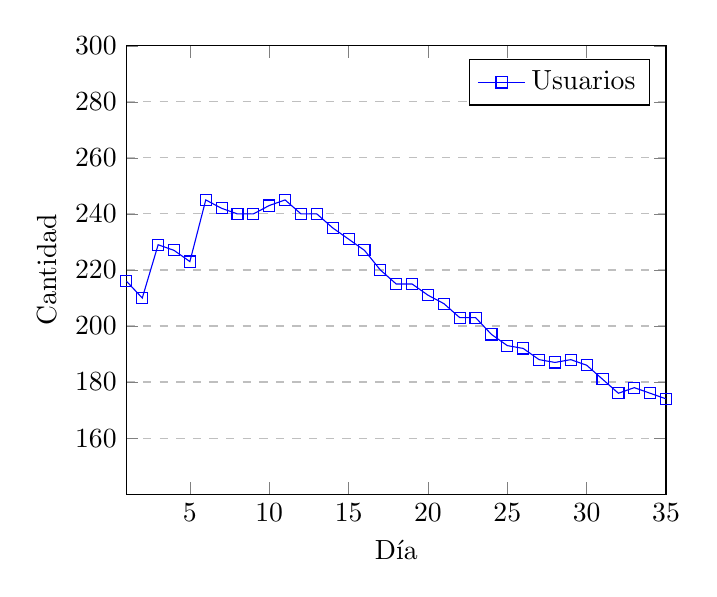
\begin{tikzpicture}
	\begin{axis}[
	xlabel={Día},
	ylabel={Cantidad},
	xmin=1, xmax=35,
	ymin=140, ymax=300,
	xtick={5,10,15,20,25,30,35},
	ytick={160,180,200,220,240,260,280,300},
	legend pos=north east,
	ymajorgrids=true,
	grid style=dashed,
	]
	
	\addplot[
	color=blue,
	mark=square,
	]
	coordinates {
		(35,174)(34,176)(33,178)(32,176)(31,181)(30,186)(29,188)(28,187)(27,188)(26,192)(25,193)(24,197)(23,203)(22,203)(21,208)(20,211)(19,215)(18,215)(17,220)(16,227)(15,231)(14,235)(13,240)(12,240)(11,245)(10,243)(9,240)(8,240)(7,242)(6,245)(5,223)(4,227)(3,229)(2,210)(1,216)
	};
	\legend{Usuarios}
	
	\end{axis}
	\end{tikzpicture}
	\caption{Cantidad de usuarios activos por día}
	\label{fig:cantidad_usuarios}
\end{figure}

Con el objetivo de caracterizar el flujo de tráfico a lo largo de una semana, se analizó la distribución de la cantidad de puntos recolectados por día de la semana y por hora del día. En la \Cref{table:localizaciones_por_dia} se puede ver la distri
bución por día de la semana, se observa que los lunes son los días en que más localizaciones se reciben, mientras que en los días domingos se recibe el menor número de localizaciones. También se puede apreciar que se recibe una mayor cantidad de localizaciones durante los días entre semana.

\begin{table}[h]
	\centering
	\begin{tabular}{ccc}
        \toprule
    	Día  & Total de Puntos & Promedio\\
    	\midrule
    	Lunes & 20262 & 4052 \\
    	Martes & 18385 & 3677 \\
    	Miércoles & 19361  & 3872 \\ 
    	Jueves & 17833 & 3567 \\
    	Viernes & 18808 & 3762 \\
    	Sábado & 16834 & 3367 \\
    	Domingo & 11936 & 2387 \\
    	\bottomrule
	\end{tabular}
	\caption{Localizaciones tomadas por día de la semana} 
	\label{table:localizaciones_por_dia}
\end{table}

En la \Cref{table:localizaciones_por_hora} se puede observar la distribución de las localizaciones durante las horas del día. Las horas con mayor cantidad de localizaciones recibidas son en la mañana de 6 a 9 y por la tarde de 17 a 19. Durante los días entre semana que son normalmente laborales, se hace más notoria esta diferencia. Mientras que durante los fines de semana la horas con mayor cantidad de localizaciones se encuentran hacia el mediodía.

\begin{table}[!h]
	\centering
	\begin{tabular}{cccc}
        \toprule
    	Hora  & Total & Entre semana & Fin de semana\\
    	\midrule
    	00 & 1947 & 1293 & 654 \\
    	01 & 1061 & 424 & 637 \\
    	02 & 1018 & 414 & 604 \\ 
    	03 & 834 & 368 & 466\\
    	04 & 821 & 424 & 397\\
    	05 & 917 & 621 & 296\\
    	06 & 5236 & 4824 & 412 \\
    	07 & 7931 & 7117 & 814\\
    	08 & 9518 & 8586 & 932\\
    	09 & 7326 & 5900 & 1426\\ 
    	10 & 4710 & 3353 & 1357\\
    	11 & 4904 & 3307 & 1597\\
    	12 & 6727 & 4489 & 2238\\
    	13 & 5636 & 3925 & 1711\\
    	14 & 5190 & 3546 & 1644\\
    	15 & 6128 & 4498 & 1630\\
    	16 & 5868 & 4418 & 1450\\ 
    	17 & 6744 & 5287 & 1457\\
    	18 & 10892 & 9204 & 1688\\
    	19 & 9639 & 8018 & 1621\\
    	20 & 7506 & 5815 & 1691\\
    	21 & 6435 & 4525 & 1910\\
    	22 & 4163 & 2933 & 1230 \\
    	23 & 2214 & 1360 & 854\\
    	\bottomrule
	\end{tabular}
	\caption{Localizaciones tomadas por hora del día} 
	\label{table:localizaciones_por_hora}
\end{table}

Otro parámetro que caracteriza el flujo de tráfico es la velocidad promedio de desplazamiento de los vehículos. En la \Cref{table:velocidad_por_hora} se observa el promedio de velocidad por hora del día. Como se aprecia en la \Cref{fig:promedio_velocidad} por las mañanas el promedio más bajo de velocidad se da entre las 6 y las 9 horas, mientras que por las tardes esto sucede de 18 a 21 horas, también se observa una disminución en la velocidad promedio durante el mediodía. En la \Cref{fig:promedio_velocidad_es_fs} se pueden apreciar las diferencias que existen en los promedios de velocidad de los días entre semana y fines de semana. Durante los días entre semana se observa un promedio menor de velocidad a partir de las 5 horas, esta velocidad promedio se mantiene menor hasta las 19 horas.

\begin{table}[h]
	\centering
	\begin{tabular}{cccc}
        \toprule
    	Hora  & Total(km/h) & Entre semana(km/h) & Fines de semana(km/h)\\
    	\midrule
    	00 & 23.2 & 22.3 & 24.9 \\
    	01 & 27.8 & 24.9 & 29.7 \\
    	02 & 30.8 & 33.1 & 29.2 \\ 
    	03 & 31.9 & 36.8 & 28.1\\
    	04 & 38.2 & 47.3 & 31.2\\
    	05 & 33.3 & 29.9 & 40.4\\
    	06 & 17.7 & 16.8 & 28.5\\
    	07 & 19.5 & 18.9 & 24.8\\
    	08 & 18.1 & 16.9 & 28.8\\
    	09 & 19.5 & 17.6 & 27.4\\ 
    	10 & 24.3 & 19.1 & 24.5\\
    	11 & 21.2 & 20.3 & 22.9\\
    	12 & 19 & 17.8 & 21.4\\
    	13 & 19.2 & 18.5 & 20.7\\
    	14 & 23.6 & 20.9 & 29.4\\
    	15 & 22.1 & 20.1 & 27.7\\
    	16 & 20.8 & 19.4 & 24.9\\ 
    	17 & 20.2 & 18.6 & 26,2\\
    	18 & 16.8 & 15.9 & 21.7\\
    	19 & 17.7 & 16.8 & 22.1\\
    	20 & 18.4 & 18.5 & 18.1\\
    	21 & 18.8 & 18.8 & 18.8\\
    	22 & 21.5 & 22.7 & 18.8\\
    	23 & 21.8 & 22.7 & 20.4\\
    	\bottomrule
	\end{tabular}
	\caption{Promedio de velocidad por hora del día} 
	\label{table:velocidad_por_hora}
\end{table}

\begin{figure}[h]
\centering
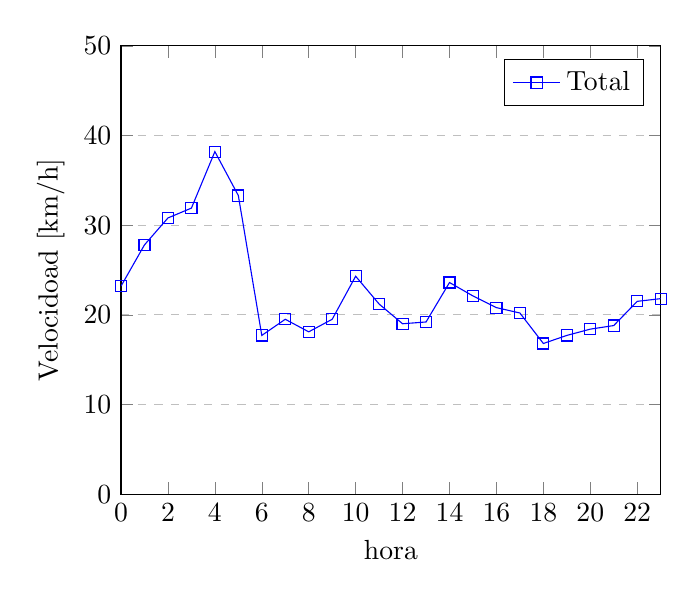
\begin{tikzpicture}
\begin{axis}[
    xlabel={hora},
    ylabel={Velocidoad [km/h]},
    xmin=0, xmax=23,
    ymin=0, ymax=50,
    xtick={0,2,4,6,8,10,12,14,16,18,20,22},
    ytick={0,10,20,30,40,50},
    legend pos=north east,
    ymajorgrids=true,
    grid style=dashed,
]
 
\addplot[
    color=blue,
    mark=square,
    ]
    coordinates {
    (0,23.2)(1,27.8)(2,30.8)(3,31.9)(4,38.2)(5,33.3)(6,17.7)(7,19.5)(8,18.1)(9,19.5)(10,24.3)(11,21.2)(12,19)(13,19.2)(14,23.6)(15,22.1)(16,20.8)(17,20.2)(18,16.8)(19,17.7)(20,18.4)(21,18.8)(22,21.5)(23,21.8)
    };
    \legend{Total}
 
\end{axis}
\end{tikzpicture}
\caption{Promedio de velocidad por hora del día}
\label{fig:promedio_velocidad}
\end{figure}

\begin{figure}[h]
\centering
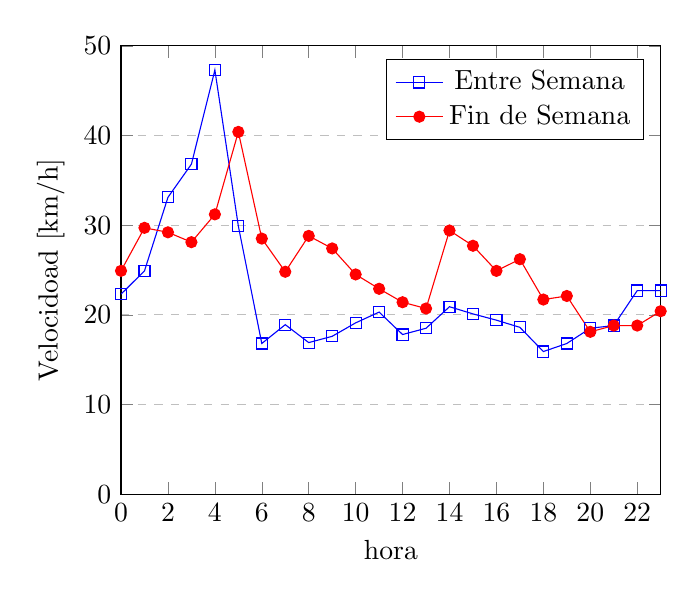
\begin{tikzpicture}
\begin{axis}[
    xlabel={hora},
    ylabel={Velocidoad [km/h]},
    xmin=0, xmax=23,
    ymin=0, ymax=50,
    xtick={0,2,4,6,8,10,12,14,16,18,20,22},
    ytick={0,10,20,30,40,50},
    legend pos=north east,
    ymajorgrids=true,
    grid style=dashed,
]
 
\addplot[
    color=blue,
    mark=square,
    ]
    coordinates {
    (0,22.3)(1,24.9)(2,33.1)(3,36.8)(4,47.3)(5,29.9)(6,16.8)(7,18.9)(8,16.9)(9,17.6)(10,19.1)(11,20.3)(12,17.8)(13,18.5)(14,20.9)(15,20.1)(16,19.4)(17,18.6)(18,15.9)(19,16.8)(20,18.5)(21,18.8)(22,22.7)(23,22.7)
    };
    \addlegendentry{Entre Semana}

\addplot[
    color=red,
    mark=*,
    ]
    coordinates {
    (0,24.9)(1,29.7)(2,29.2)(3,28.1)(4,31.2)(5,40.4)(6,28.5)(7,24.8)(8,28.8)(9,27.4)(10,24.5)(11,22.9)(12,21.4)(13,20.7)(14,29.4)(15,27.7)(16,24.9)(17,26.2)(18,21.7)(19,22.1)(20,18.1)(21,18.8)(22,18.8)(23,20.4)
    };
    \addlegendentry{Fin de Semana}
 
\end{axis}
\end{tikzpicture}
\caption{Comparativa de Promedio de velocidad por hora del día}
\label{fig:promedio_velocidad_es_fs}
\end{figure}

El resultado del análisis de tráfico puede ser observado en tiempo real por los usuarios de la aplicación móvil, o accediendo a accediendo a la aplicación web desarrollada para el efecto. En la \Cref{fig:trafico_lunes} se puede observar un ejemplo del estado del tráfico observado en un día lunes a las 9 de la mañana, como se puede ver existe una gran cantidad de calles con niveles de velocidad bajo. La \Cref{fig:trafico_sabado} corresponde al estado del tráfico observado un día sábado a las 9 de la mañana, se puede apreciar que existe una menor cantidad de información y que los niveles de velocidad son más variados con relación a un día lunes a la misma hora, esto se debe a que durante los fines de semana se registra una menor cantidad de localizaciones.

\begin{figure}[!ht]
	\centering
	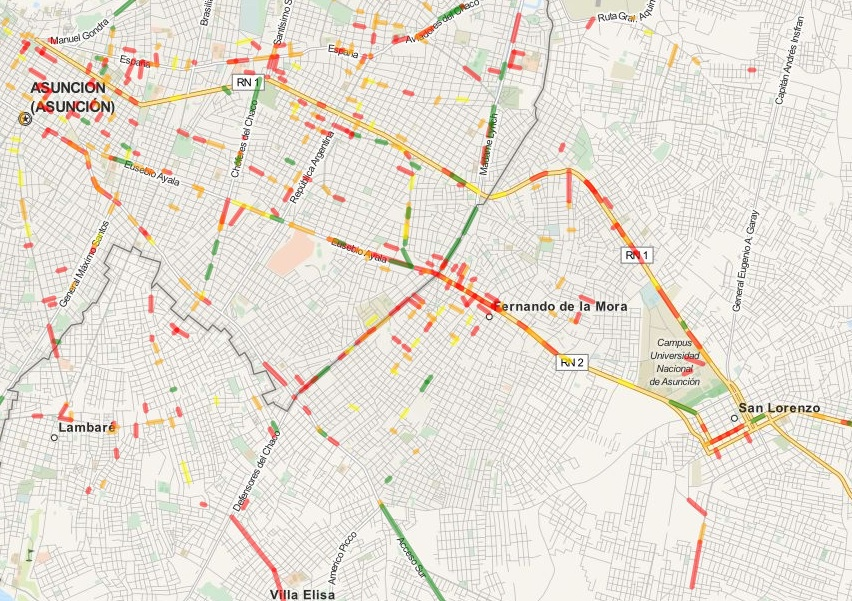
\includegraphics[width=0.7\textwidth]{capitulos/7/figuras/figura6.jpg}
	\caption{\label{fig:trafico_lunes} Tráfico en día lunes a las 9 am}	
\end{figure}

\begin{figure}[!ht]
	\centering
	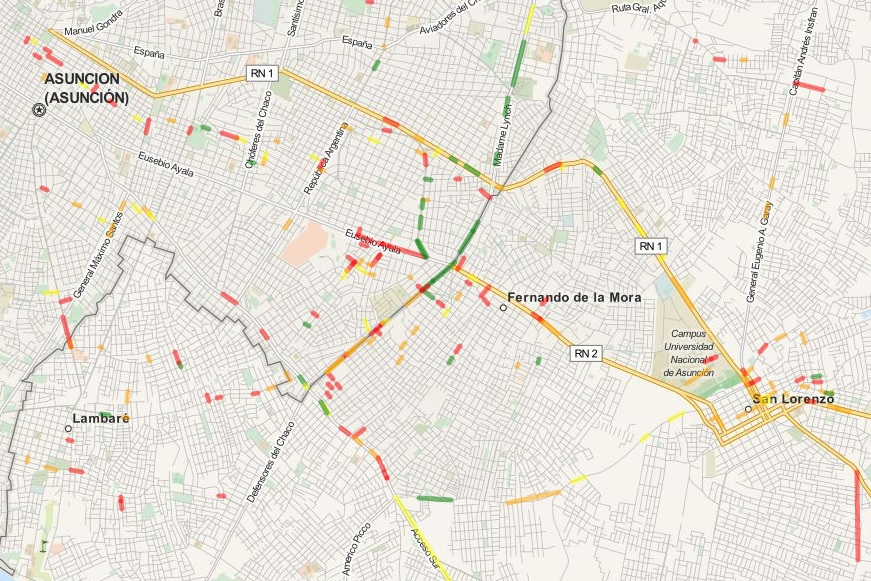
\includegraphics[width=0.7\textwidth]{capitulos/7/figuras/figura7.jpg}
	\caption{\label{fig:trafico_sabado} Tráfico en día sábado a las 9 am}	
\end{figure}


